\documentclass[tikz,border=10pt]{standalone}
\usepackage{amsmath}
\usepackage{amssymb}
\usepackage{tikz}
\usetikzlibrary{arrows.meta,calc}

\definecolor{figazul}{RGB}{2,132,199}
\definecolor{figrojo}{RGB}{220,38,38}
\definecolor{figverde}{RGB}{22,163,74}

\begin{document}
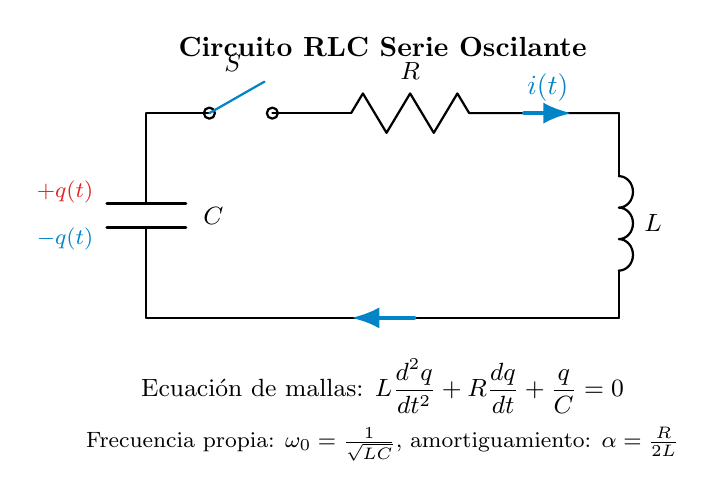
\begin{tikzpicture}[>=Latex, line cap=round, line join=round]
  % Título / encabezado del circuito
  \node[above, font=\bfseries] at (3.0, 3.2) {Circuito RLC Serie Oscilante};

  % Malla rectangular del circuito RLC
  % Esquinas: (0,0), (6.0, 0), (6.0, 2.6), (0, 2.6)

  % Rama superior: Interruptor S y Resistencia R
  \draw[thick] (0, 2.6) -- (0.8, 2.6);
  % Interruptor S (abierto o cerrándose)
  \draw[thick] (0.8, 2.6) circle (2pt);
  \draw[thick] (1.6, 2.6) circle (2pt);
  \draw[thick, color=figazul] (0.8, 2.6) -- (1.5, 3.0);
  \node[above, font=\small] at (1.1, 3.0) {$S$};

  \draw[thick] (1.6, 2.6) -- (2.6, 2.6);
  % Resistor R (zigzag)
  \draw[thick] (2.6, 2.6) -- (2.75, 2.85) -- (3.05, 2.35) -- (3.35, 2.85) -- (3.65, 2.35) -- (3.95, 2.85) -- (4.1, 2.6) -- (6.0, 2.6);
  \node[above, font=\small] at (3.35, 2.9) {$R$};

  % Rama derecha: Inductor L (bobinas / bucles verticales)
  \draw[thick] (6.0, 2.6) -- (6.0, 1.8);
  \draw[thick] (6.0, 1.8) arc (90:-90:0.18 and 0.2) arc (90:-90:0.18 and 0.2) arc (90:-90:0.18 and 0.2);
  \draw[thick] (6.0, 0.6) -- (6.0, 0);
  \node[right, font=\small] at (6.2, 1.2) {$L$};

  % Rama inferior: conductor de retorno
  \draw[thick] (6.0, 0) -- (0, 0);

  % Rama izquierda: Capacitor C con placas paralelas
  \draw[thick] (0, 0) -- (0, 1.15);
  % Placa inferior
  \draw[very thick] (-0.5, 1.15) -- (0.5, 1.15);
  % Placa superior
  \draw[very thick] (-0.5, 1.45) -- (0.5, 1.45);
  \draw[thick] (0, 1.45) -- (0, 2.6);

  % Carga +q(t) y -q(t) en las placas
  \node[left, font=\footnotesize, color=figrojo] at (-0.55, 1.6) {$+q(t)$};
  \node[left, font=\footnotesize, color=figazul] at (-0.55, 1.0) {$-q(t)$};
  \node[right, font=\small] at (0.6, 1.3) {$C$};

  % Flecha de corriente i(t) en sentido horario
  \draw[->, ultra thick, color=figazul] (4.8, 2.6) -- (5.4, 2.6) node[above, midway, color=figazul] {$i(t)$};
  \draw[->, ultra thick, color=figazul] (3.4, 0) -- (2.6, 0);

  % Ecuación diferencial del circuito (Ley de Kirchhoff de voltajes)
  \node[below, font=\small, align=center] at (3.0, -0.4) {
    Ecuaci\'on de mallas: $\displaystyle L\frac{d^2q}{dt^2} + R\frac{dq}{dt} + \frac{q}{C} = 0$ \\[4pt]
    \footnotesize Frecuencia propia: $\omega_0 = \frac{1}{\sqrt{LC}}$, amortiguamiento: $\alpha = \frac{R}{2L}$
  };

\end{tikzpicture}
\end{document}
